\documentclass[10pt, letterpaper]{article}
\usepackage[cm]{fullpage}
\usepackage{algpseudocode}
\usepackage{algorithm}
\usepackage{graphicx}
\usepackage[section]{placeins}
\usepackage[table]{xcolor}
\usepackage{amsmath}
\usepackage[margin=1in]{geometry}


\algrenewcommand\Return{\State \algorithmicreturn{} }%


\title{Largest Subarray}
\author{Daiwei Chen \and Joseph Watts}

\begin{document}
	\maketitle
	\begin{abstract}
		Calculating the maximum sum of values within a contiguous subset of an array is a problem mostly found in the field of image processing. 
		This paper explores the impact of using two different approaches to solve this problem.One approach is using a brute force algorithm, and the other is using a more optimized approach known as Kadane's algorithm.
		Due to the different complexity of these two algorithms used to solve it,
		we will see the performance impact over a range of different sized arrays.
	\end{abstract}
	\section{Background and Related Work}
  Finding the largest subarray is a problem where we have to find an subarray within a given list $L$. And make sure that the found subarray has a sum higher than any other possible subarrays within $L$.
  This algorithm is important and has some real world uses. One such as computer vision, to find the brightest area within an image, it's basically a ``Maximum Subarray'' problem on the lumens within the list of pixels.

	\subsection{Brute Force Algorithm}

	\begin{algorithm}
	\begin{algorithmic}
		\caption{Brute Force}\label{bruteforce}
	\Function{bruteForce}{A}
	\State $n\gets len(A)$
	\State $maxsum\gets A[0]$
	\For{$i$ in 0..$n$-1}
	\For{$j$ in $i$..$n$-1}
	\State $total\gets 0$
	\For{$k$ in $i$..$j$}
	\State $total\gets total + A[k]$
	\EndFor
	\If{$maxsum < total$}
	\State $maxsum\gets total$
	\EndIf
	\EndFor
	\EndFor
	\EndFunction
	\end{algorithmic}
	\end{algorithm}


	This brute force algorithm works by keeping track of both a start and ending index, and then calculating a sum for all the indexes between.
%	This brute force algorithm works by keeping track of two main index values.
%	The first index is for the outer loop which will run between 0 and the number of elements in the array, while the second keeps track of the ending index and runs between the starting index and the number of elements in the array.
%	This will allow for the capture of every possible subset of the array.
%	The second index will contain a value between the first index value used by the outer loop and the number of elements in the array.
%	A value to keep track of the sum of our array is made and then the array is summed between the two indexes.
%	If our summed value is higher than our highest previously summed value, then update it to the new value.
%	At this point the second index will be incremented, causing the sum between the indexes to take place again.


	% Summation Equation
	\[\sum_{i = 0}^{n-1}\sum_{j = i}^{n-1}\sum_{k = i}^{j}1\]
  \begin{equation}
    \begin{split}
      \sum_{i=1}^{n}&\sum_{j=1}^{i}\sum_{k=j}^{i+j}1 \\
      &=\sum_{i=1}^{n}\sum_{j=1}^{i}i+1 \\
      &=\sum_{i=1}^{n}\sum_{j=1}^{i}i+\sum_{j=1}^{i}1 \\
      &=\sum_{i=1}^{n}\frac{i(i+1)}{2}+i \\
      &=\sum_{i=1}^{n}(\frac{1}{2}i^2+\frac{i}{2})+\sum_{i=1}^{n}i \\
      &=\frac{1}{2}\sum_{i=1}^{n}i^2+\frac{1}{2}\sum_{i=1}^{n}i+\sum_{i=1}^{n}i \\
      &=\frac{1}{2}*\frac{1}{6}n(n+1)(2n+1)+\frac{1}{2}\frac{n(n+1)}{2}+\frac{n(n+1)}{2} \\
      &=\frac{1}{12}n(2n^2+3n+1)+\frac{(n^2+n)}{4}+\frac{2(n^2+n)}{4} \\
      &=\frac{1}{6}n^3+\frac{1}{4}n^2+\frac{1}{12}n+\frac{3(n^2+n)}{4} \\
      &=\frac{1}{6}n^3+\frac{1}{4}n^2+\frac{1}{12}n+\frac{3n^2+3n}{4} \\
      &=\frac{1}{6}n^3+n^2+\frac{10}{12}n \\
    \end{split}
  \end{equation}

	The starting index goes from the position of the first element until the last element, while the ending index repeats for all values between the starting index and the position of the last element.
	A third loop then sums all the values found between these two indexes.

	The outer loop keeps track of $i$, the starting index, and runs the entire length of the array, or $n$ times.
	The middle loop keeps track $j$, the ending index, and runs the length between $i$ and the end of the array, $n$.
	There is then another inner value, $k$, which runs between the values of $i$ and $j$.

	Due to these three nested summations, the brute force algorithm runs in $O(n^3)$ time.
	It should be noted, however, that there is a slightly different version of this brute force algorithm that runs in $O(n^2)$ time by doing the sum as part of the second loop.

	\subsection{Kadane Algorithm}

  \begin{algorithm}
		\caption{Kadane Algorithm}\label{kadane}
	\begin{algorithmic}
	  \Function{Kadane}{L}
    \State $maxEnding \gets L[0]$
    \State $maxAlways \gets L[0]$
    \For{i 1..len(L)}
    \State $maxEnding \gets \Call{max}{L[i], maxEnding + L[i]}$
    \State $maxAlways \gets \Call{max}{maxAlways, maxEnding}$
    \EndFor
	  \Return{$maxAlways$}
	  \EndFunction
	\end{algorithmic}
	\end{algorithm}
  Kadane is a very good example of a simple but effective way to write a better algorithm using dynamic programming. It focuses on remembering two very important variables $maxEnding$ and $maxAlways$. $maxAlways$ will always remember the largest sum you've seen up till now out of all the subarrays. But $maxEnding$ will keep track of the largest subset just within that iteration of i. Because it remembers what sort of sums you've checked before, you do not have to check other possible subarrays again. Thus getting rid of the 2 for loops within the brute force algorithm.

  \[
  \sum_1^n2 \\
  = 2 * n \\
  = \Theta(n)
		\]
	This algorithm has a big $\Theta$ of n because it only goes through each element of the array once and only once.
	\section{Experimental Setup}
	For the experimental setup, we have allowed our users to either input an array to test both algorithms against, or run our own tests.
  Our own tests included of multiple n values that will be timed. For each n value, we randomly generate n numbers of numbers between -5 and 5 inclusive and place them into a list. We then will time each run of the brute force algorithm and kadane algorithm to go through that list of random numbers. After about 100 trials for each n, we will collecte all the timing data and proceed to find the averge run time for both algorithms for that n.
  Timing data is collected by using a high definition clock within Rust. These timings were done on an Intel Xenon X5570 processor clocked at 2.9GHz. The host machine was running a 64bit version of Fedora 29 Server Edition.
	\section{Results}
	Include our graph visualization of our data here. Brute Force and Kadane Timing


	% Add the graph showing the time taken.
	\begin{figure}[!htb]
	\center{
		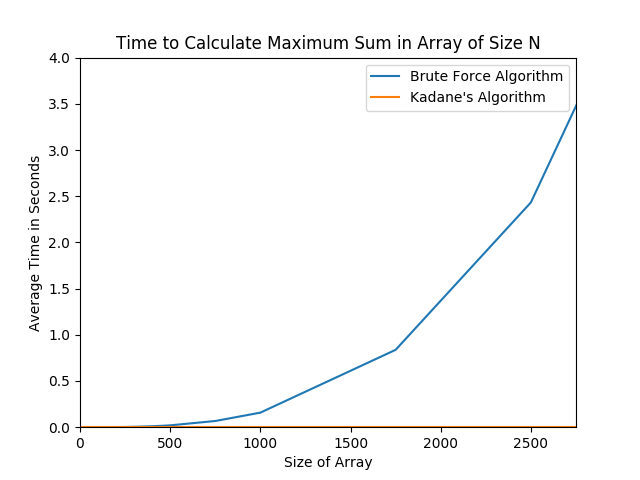
\includegraphics[width=0.75\textwidth] {python/avgTimeGraph.png}
	}
	\caption{
		\label{fig:time-graph} Graph of Brute Force vs Kadane Timings
	}
	\end{figure}

	% Add a table showing the time taken.

	\begin{figure}[!htb]
	\begin{center}
	\caption{
		\label{fig:time-table} Table of Brute Force vs Kadane Timings
	}
	\medskip
	\begin{tabular}{ | p{2cm} | l | l | }
			\hline
			Size of Array & Brute Force (s) & Kadane (s) \\ \hline
			1 & 0.000000033 & 0.000000025 \\ \hline
			5 & 0.000000085 & 0.000000036 \\ \hline
			10 & 0.000000448 & 0.000000051 \\ \hline
			50 & 0.000030930 & 0.000000125 \\ \hline
			100 & 0.000194367 & 0.000000184 \\ \hline
			150 & 0.000594095 & 0.000000260 \\ \hline
			200 & 0.001366055 & 0.000000331 \\ \hline
			250 & 0.002607847 & 0.000000402 \\ \hline
			300 & 0.004420136 & 0.000000466 \\ \hline
			350 & 0.006950275 & 0.000000573 \\ \hline
			400 & 0.010421218 & 0.000000639 \\ \hline
			450 & 0.014655456 & 0.000000716 \\ \hline
			500 & 0.020030729 & 0.000000956 \\ \hline
			750 & 0.067125954 & 0.000001231 \\ \hline
			1000 & 0.157617270 & 0.000001779 \\ \hline
			1750 & 0.837418008 & 0.000002682 \\ \hline
			2500 & 2.432867191 & 0.000003601 \\ \hline
			3500 & 6.606255604 & 0.000005064 \\ \hline
		\end{tabular}
	\end{center}
\end{figure}
	\section{Conclusions}
	As cleary shown through our graph and time table found in Section 3,
	Kadane's algorithm is a much more optimized solution to solve the problem of finding the maximum sum of values within an array.
	A brute forcing algorithm can be simplified down to $O(n^2)$, but our algorithm runs in $O(n^3)$.
	At the same time Kadane's algorithm runs in $O(n)$ time meaning that it will execute much faster.
	The amount of time that this algorithm saves is exponential.
	\end{document}
